
\documentclass[handout]{beamer} % [notesonly] [notes]
%\documentclass[slidestop,compress,mathserif]{beamer}
%%\usepackage[bars]{beamerthemetree} % Beamer theme v 2.2
\usetheme{Antibes} % Beamer theme v 3.0
%\usecolortheme{lily} % Beamer color theme %lily, beaver
%\usecolortheme{default}% schwarz, dunkelblau, blau
%\usecolortheme{sidebartab} % schwarz, dunkelblau, blau
%\usecolortheme{albatross} %nix
%\usecolortheme{beetle} 
%\usecolortheme{crane}
%\usecolortheme[named=SeaGreen]{dove} % keine farbe
%\usecolortheme{fly} % grauer hintergrund
%\usecolortheme{seagull} %grau

% http://www.matthiaspospiech.de/latex/vorlagen/beamer/preambel/beamer-settings/3/

\usecolortheme{dove}
\usefonttheme{default}

%\usecolortheme[named=SeaGreen]{orchid} % gut
%\usecolortheme{structure} % schwarz

%\usepackage[T1]{fontec}		%deutsche silbentrennung
%\usepackage[applemac]{inputenc}	%um Umlaute korrekt schreiben zu knnen


\usepackage[T1]{fontec}		%deutsche silbentrennung
\usepackage[applemac]{inputenc}	%um Umlaute korrekt schreiben zu knnen

\usepackage[german]{babel}		%deutsche silbentrennung
\usepackage[ansinew]{inputenc}	%um Umlaute korrekt schreiben zu knnen
\usepackage{amssymb,amsmath}
\usepackage{graphicx}
\usepackage{hyperref}
\usepackage{here}
\usepackage{color}
\usepackage{pdfpages}			%kann mit pdfpage{xxx.pdf} pdfs einbinden
\usepackage{float}                 %damit Bild an dem Ort, wo es sein soll
\restylefloat{figure}              %damit Bild an dem Ort, wo es sein soll


\usepackage{tikz}
\usetikzlibrary{mindmap,trees}


%% handout
%% -----
%\usepackage{pgfpages} 
%\pgfpagesuselayout{2 on 1}[a4paper,border shrink=5mm] 


%% define colors
%% --------
%\definecolor{my}{rgb}{0.20,0.43,0.09}

%\usetheme{} 
%\setbeamercovered{transparent}
%\setbeamercolor{palette primary}{fg=black,bg=my} % !<#> is transparency
%\setbeamercolor{palette secondary}{fg=black,bg=my!60  }
%\setbeamercolor{palette tertiary}{fg=black,bg=my!60!gray }
%\setbeamercolor{palette quaternary}{fg=black,bg=my!60!black}



\setbeamertemplate{footline}[frame number]

\title{Visualizing Data}
\author{Sina R�eger}
\institute{Institute of Data Analysis and Process Design (IDP)}
%\institute{Z�rcher Hochschule f�r Angewandte Wissenschaften \\ 
%Institut f�r Datenanalyse und Prozessdesign}

% .........................................................................

\begin{document}

% .........................................................................

\frame{
  \titlepage
} 
%% ===========================================================
%% E I N S T I E G

\section{Introduction}

  
%\subsection{Aspekte}
%% --------
 \frame{
  \frametitle{Example: temperature in train}
     \begin{figure}[H]
   	\centering
    	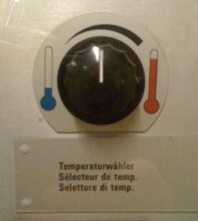
\includegraphics[width=6cm]{images/IMG_0066b.jpg}
     \end{figure}
  }
   \note[options]{Ein Temperaturw�hler in der S12. Hier sieht man etwas, was auch bei statistischen Grafiken oft geschieht: doppelte Information - Redundanz. Im Prinzip h�tten wir gleich viel Information, wenn wir nur die Farben oder nur die Thermometerh�he wissen w�rden. Dass die Information doppelt ist, hat den Grund, dass das Auge die Information besser verarbeiten und erkennen kann. Bei statistischen Grafiken allerdings muss aufgepasst werden, dass diese Redundanz nicht geschieht, weil das Auge dann fehlgeleitet werden kann. Eine statistische Grafik soll so wenig Dimensionen haben, wie der Datensatz.}

  

%% ===========================================================
\section{Aspects of visualizing data}


%% -------- 3 schwarze Menschen
 \frame{
  \frametitle{Three aspects}
     \begin{figure}[H]
   	\centering
     	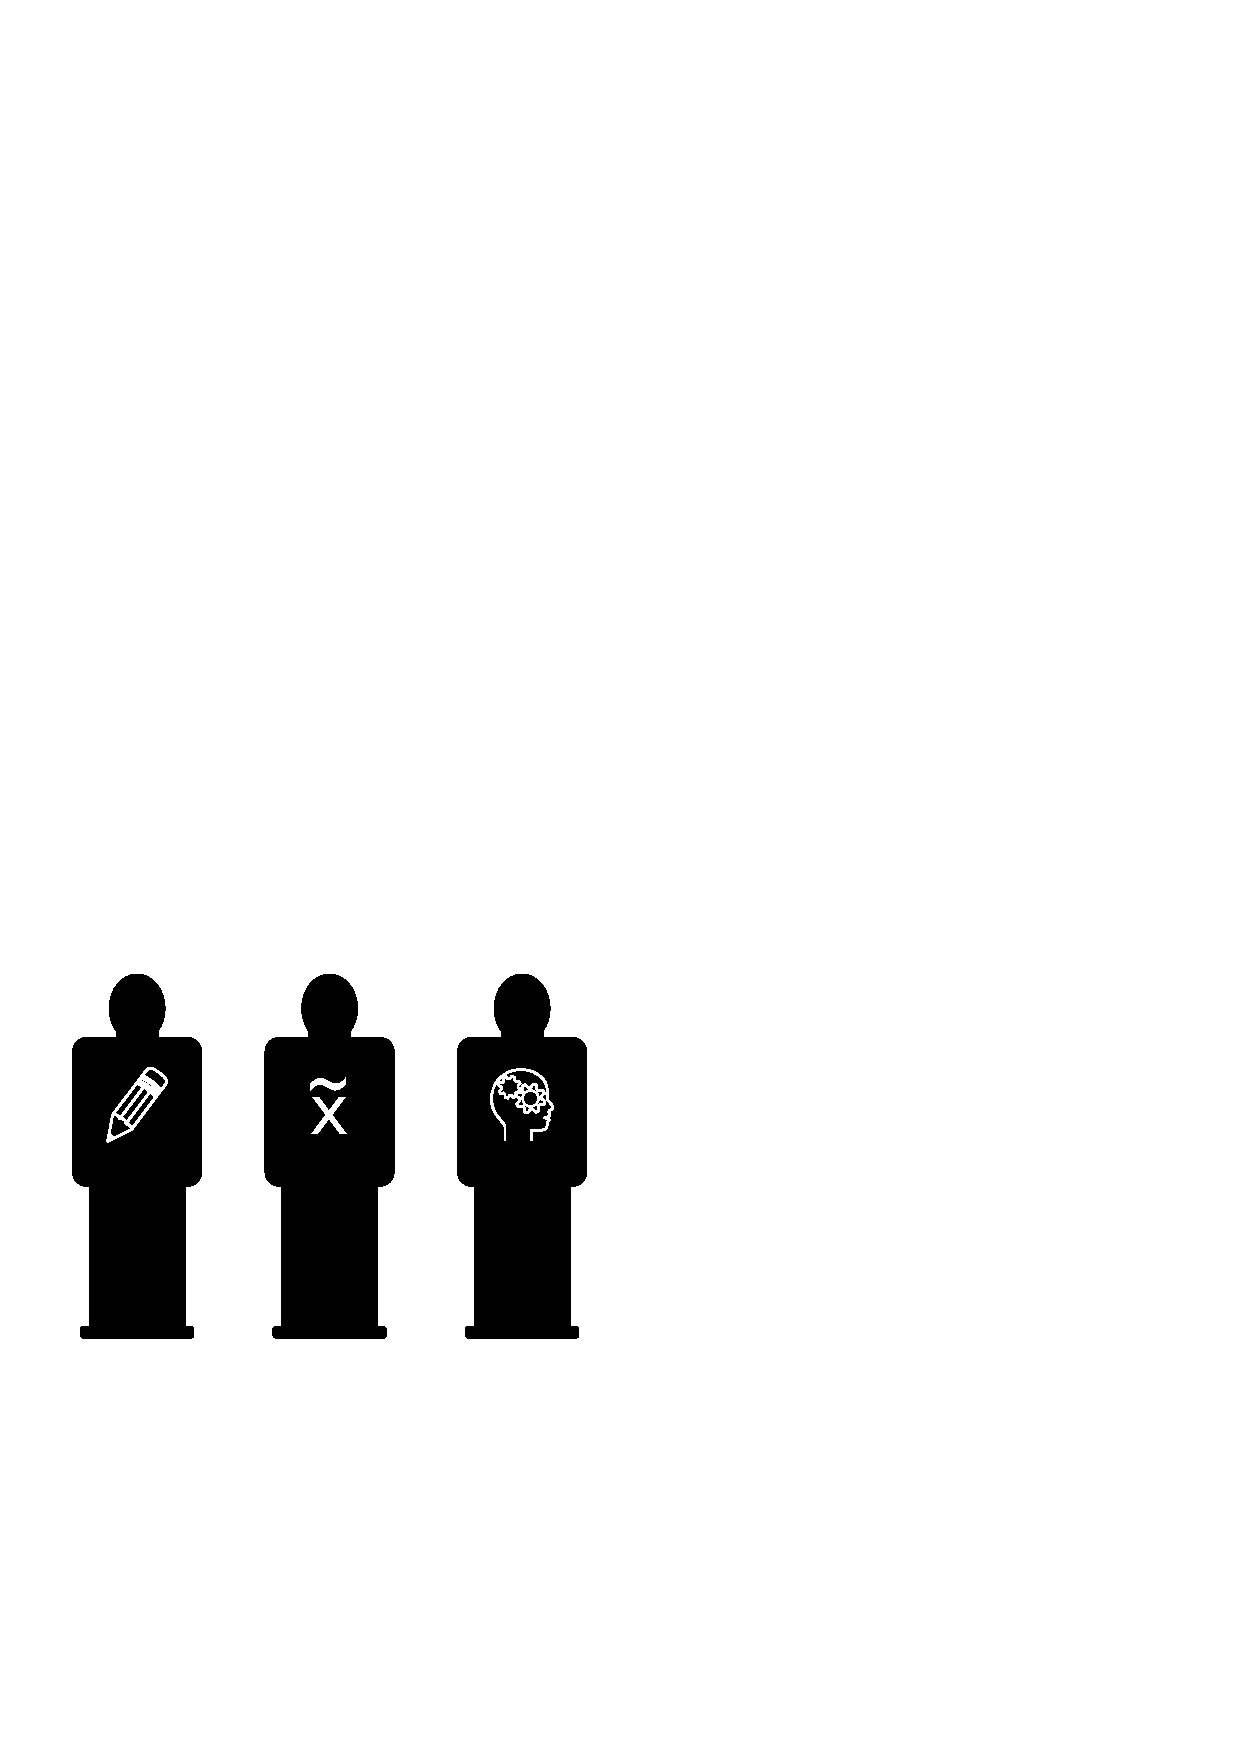
\includegraphics[width=8cm]{images/Zeichnung2.pdf}
     \end{figure}
     
     \begin{center}
     {\footnotesize After isotype, Otto Neurath, 1882 -- 1945}
     \end{center}

}
  \note[options]{Die drei Menschen repr�sentieren die drei Aspekte einer Visualisierung.
  		\item GrafikerIn: weiss wie man gestaltet / Unterhaltung
 		\item StatistikerIn: aggregiert Zahlen, bestimmt die Art der Grafik (Histogramm, etc.)
		\item PsychologIn: weiss, wer was versteht, Adressierung, Arbeitsgrafik oder Pr�sentationsgrafik
		
Die drei Aspekte h�ngen alle zusammen. Design hat mit wahrnehmung zu tun, statisitk mit design und wahrnehmung. Und nat�rlich setzt das alles auch ein Wissen �ber die Substanz voraus.

   Eine gute Visualisierung von Zahlen ist gestaltet, richtig addressiert und beinhaltet die richtige Statistik. Wir alle sind vermutlich eher Statistiker, f�r die Gestaltung m�ssten wir eine entsprechende Ausbidlung absolcvieren. Manchmal gehen Aspekte verloren oder der Fokus darauf. Um zu verdeutlichen, was mit diesen drei aspekten gemeint, ist, habe ich je zwei Beispiele gemacht.}

%% -------- Beispiel GrafikerIn
 \frame{
  \frametitle{Example graphic designer}
\begin{figure}[H] 
    \centering 
       \subfloat{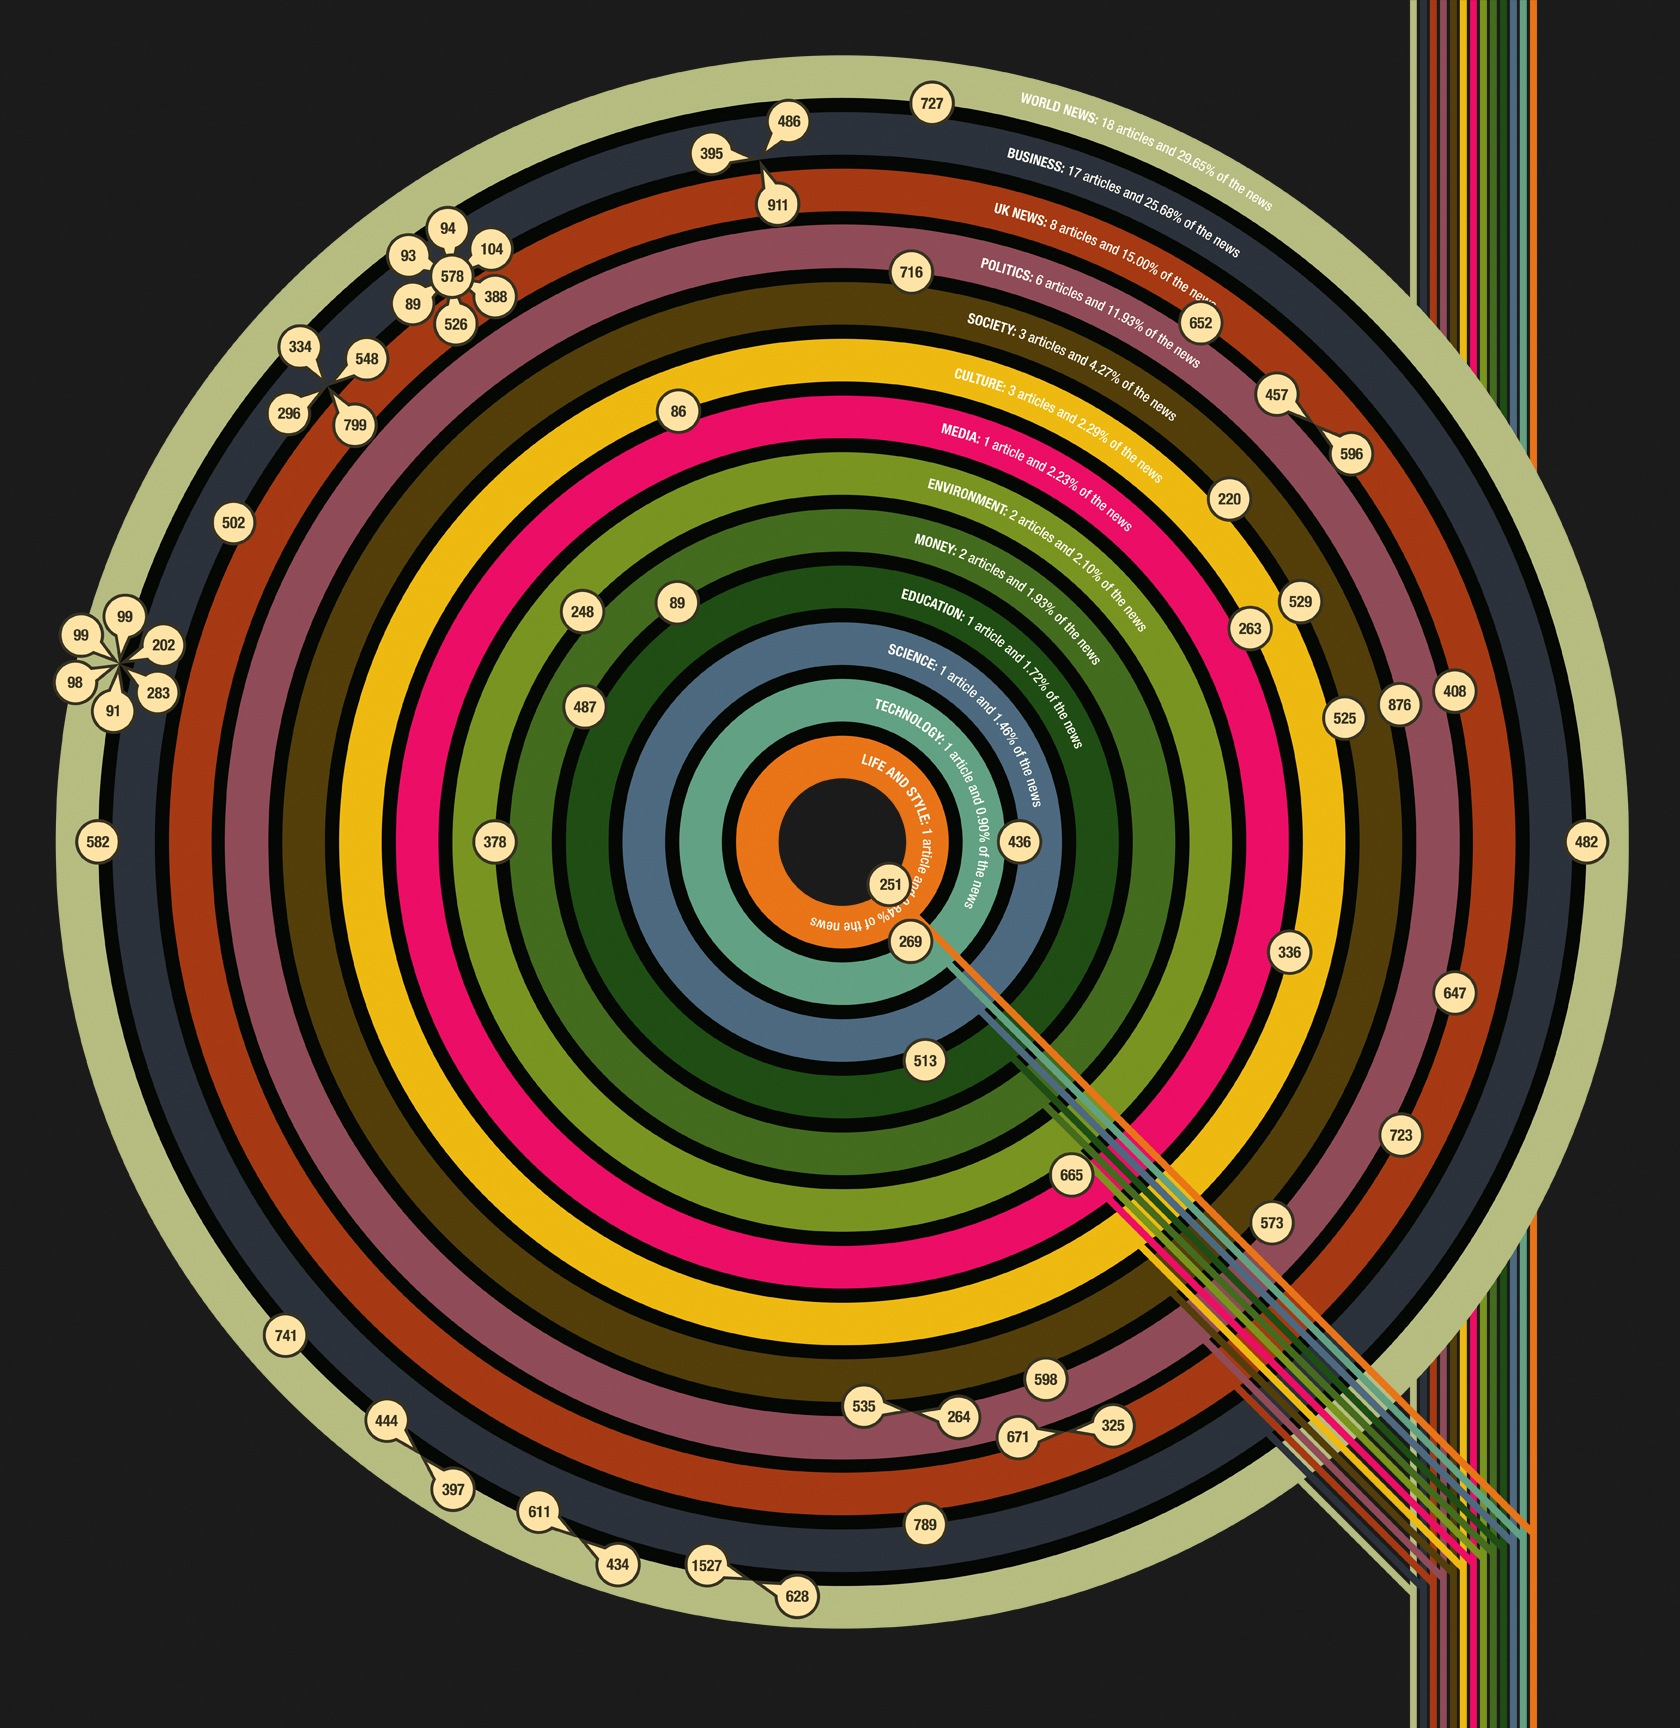
\includegraphics[width=5cm]{Images/One_week_of_the_guardian1a.jpg}}
        \subfloat{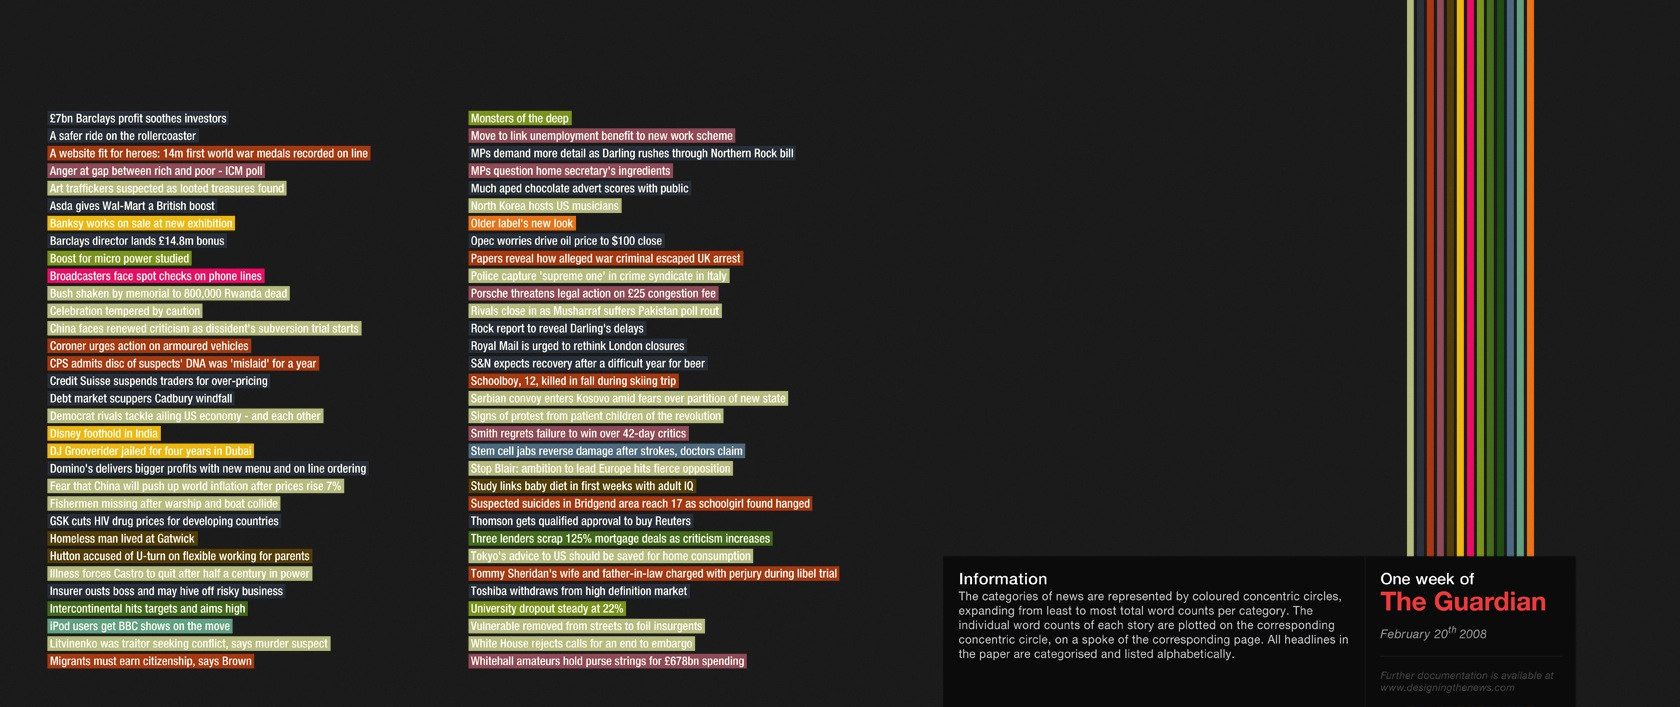
\includegraphics[width=5cm]{Images/One_week_of_the_guardian1b.jpg}}
 \end{figure}
       \begin{center}
     {\footnotesize One Week of The Guardian - Designing the News.}
          {\tiny (http://www.designingthenews.com/wp-content/uploads/2008/04/03\_wednesday\_a1\_72.jpg, letzter Zugriff: 2009-01-07)}
    \end{center}
  
    
}
  \note[options]{OverKill in Design: Beispiel aus Data-Flow. Ausgeglichene Grafik: verbesserte Grafik}

%% -------- Beispiel StatisikerIn
 \frame{
  \frametitle{Example statistician}
\begin{figure}[H] 
   \centering 
        \subfloat{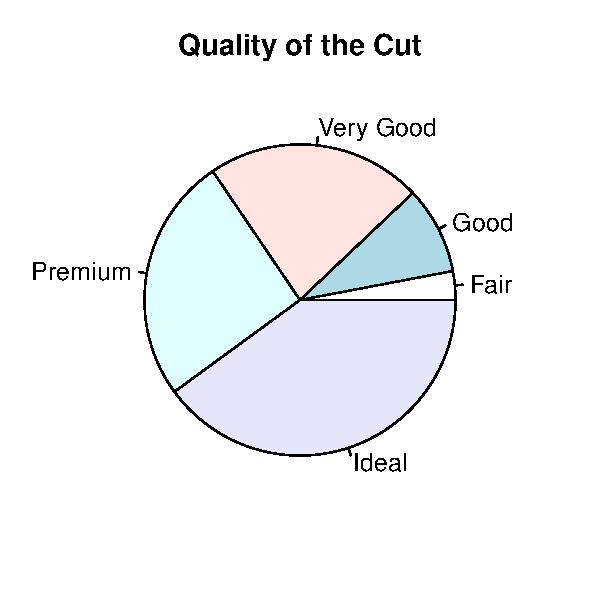
\includegraphics[width=5cm]{Images/pie.pdf}}
        \subfloat{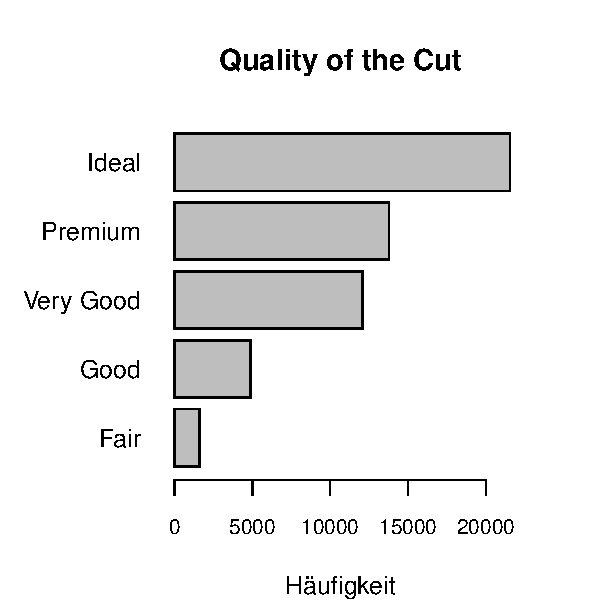
\includegraphics[width=5cm]{Images/barplot.pdf}}
  \end{figure}
       \begin{center}
     {\footnotesize Piechart and barplot of diamonds data.}
     \end{center}

}
  \note[options]{Falsche Statistik: Kuchendiagramm statt Barplot}


%% -------- Beispiel PsychologIn
 \frame{
  \frametitle{Example psychologist}
\begin{figure}[H] 
    \centering 
        \subfloat{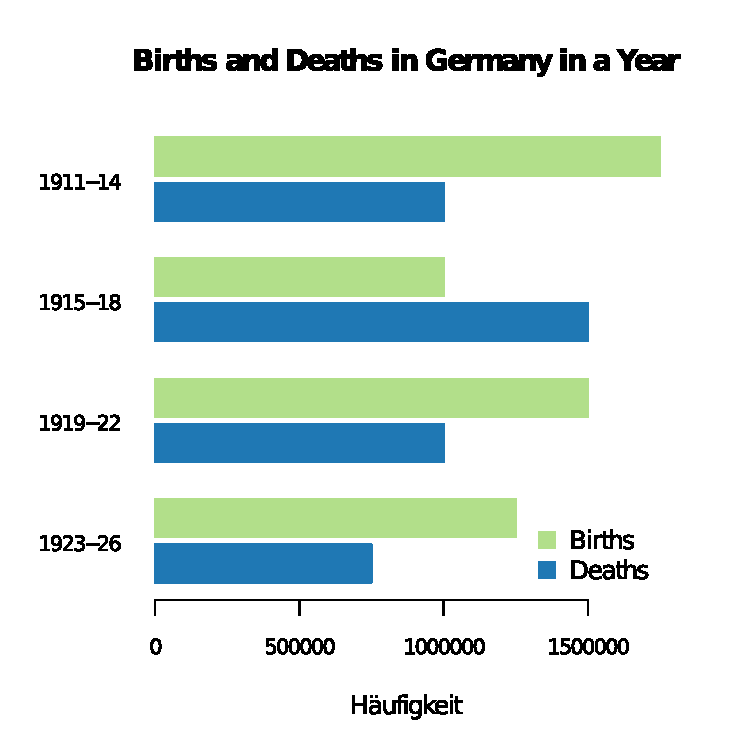
\includegraphics[width=5cm]{Images/barplot_birth_deaths2.pdf}}
        \subfloat{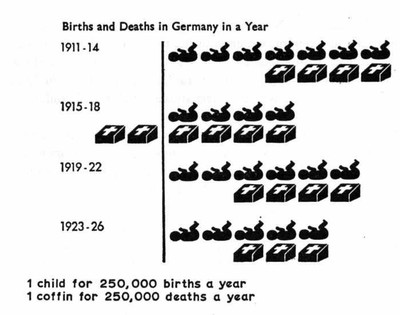
\includegraphics[width=5cm]{Images/neurath_birth_death.jpg}}
\end{figure}
      \begin{center}
     {\footnotesize Birth and deaths in germany: barplot and pictogramms.}\\
     {\scriptsize (http://www.latebytes.nl/archives/2008/04/17/T1\_N112\_A6\_Isotype-Neurath.jpg, last access: 2011-11-29)}
     \end{center}
}



%% ===========================================================
%% W A H R N E H M U N G 
\section{Visual perception}


%% --------
 \frame{
  \frametitle{Processing information}
  
  \begin{figure}[H] 
    \centering 
	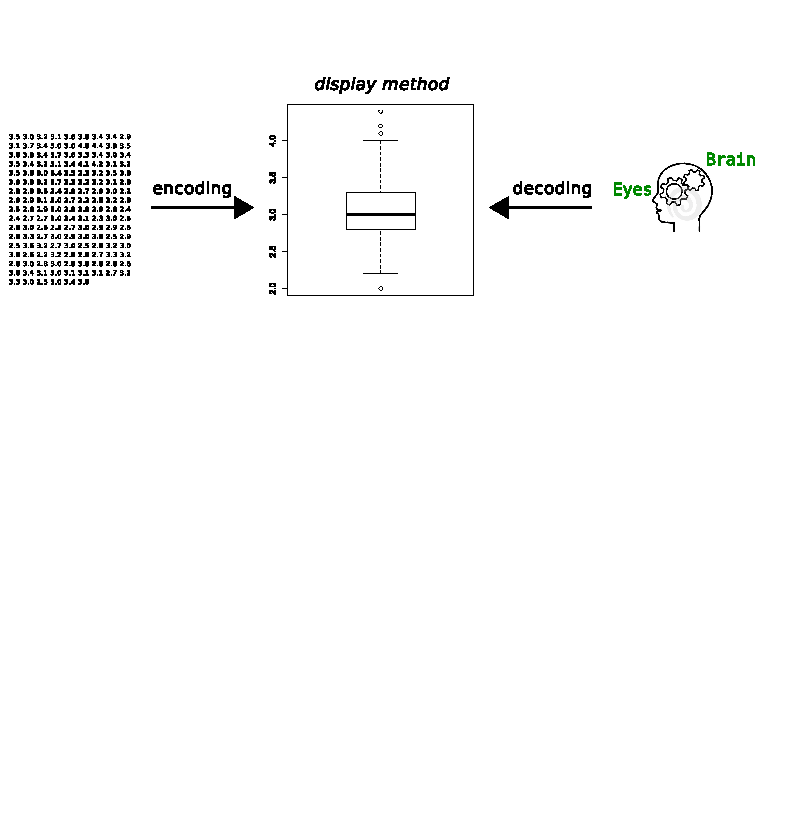
\includegraphics[width=11cm]{Images/wahrnehmung_kursiv2.pdf}
\end{figure}

  	 \begin{block}{Encoding}
	Graph data = encode information
	\end{block}
	
	 \begin{block}{Decoding}
      	Visual perception = decode information
	\end{block}
     {\scriptsize \emph{The Elements of Graphing} from William S. Cleveland (1994)}
}




%% --------
 \frame{
  \frametitle{}
 \begin{figure}[H] 
    \centering 
       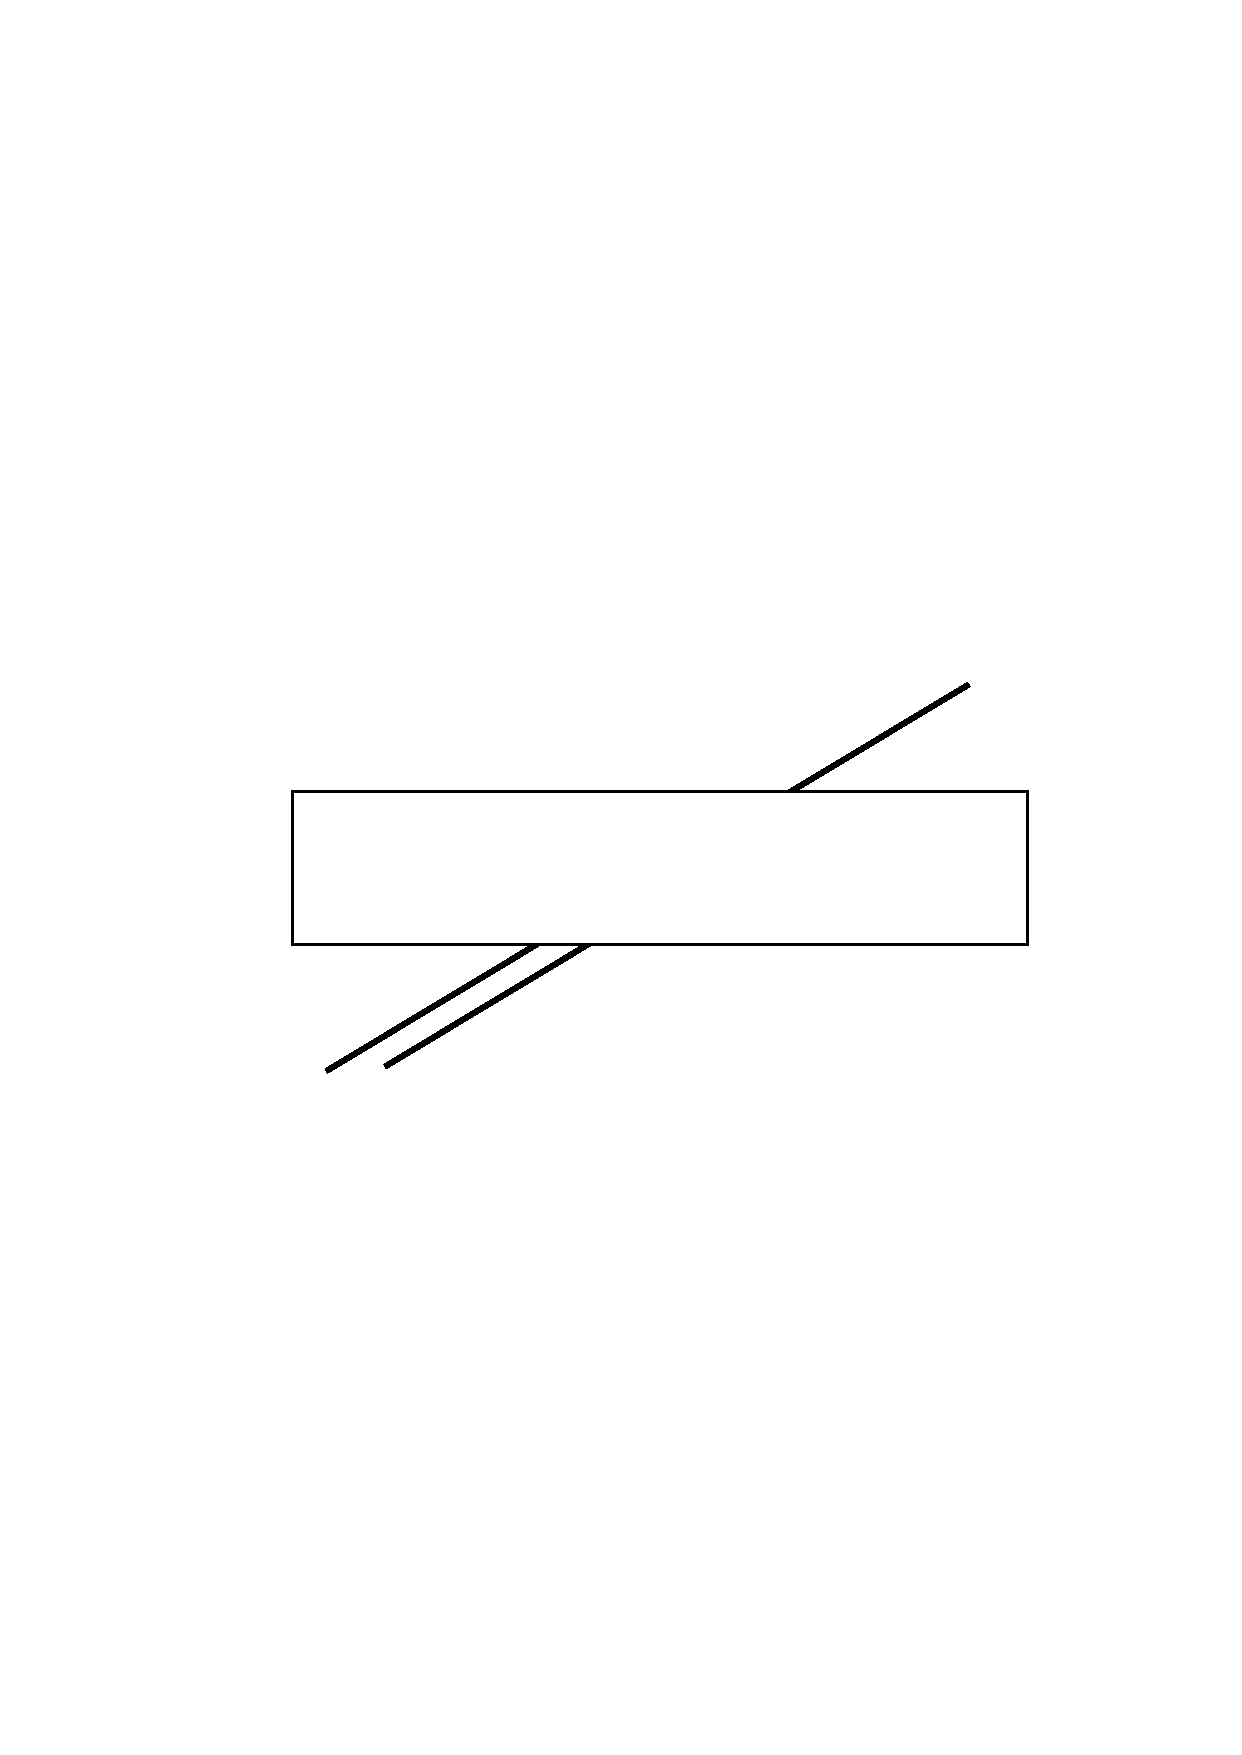
\includegraphics[width=9cm]{Images/optische_taeuscung2.pdf}
\end{figure}
       \begin{center}
     {\footnotesize  Poggendorff illusion}
     \end{center}
}

%% --------
 \frame{
  \frametitle{}
 \begin{figure}[H] 
    \centering 
       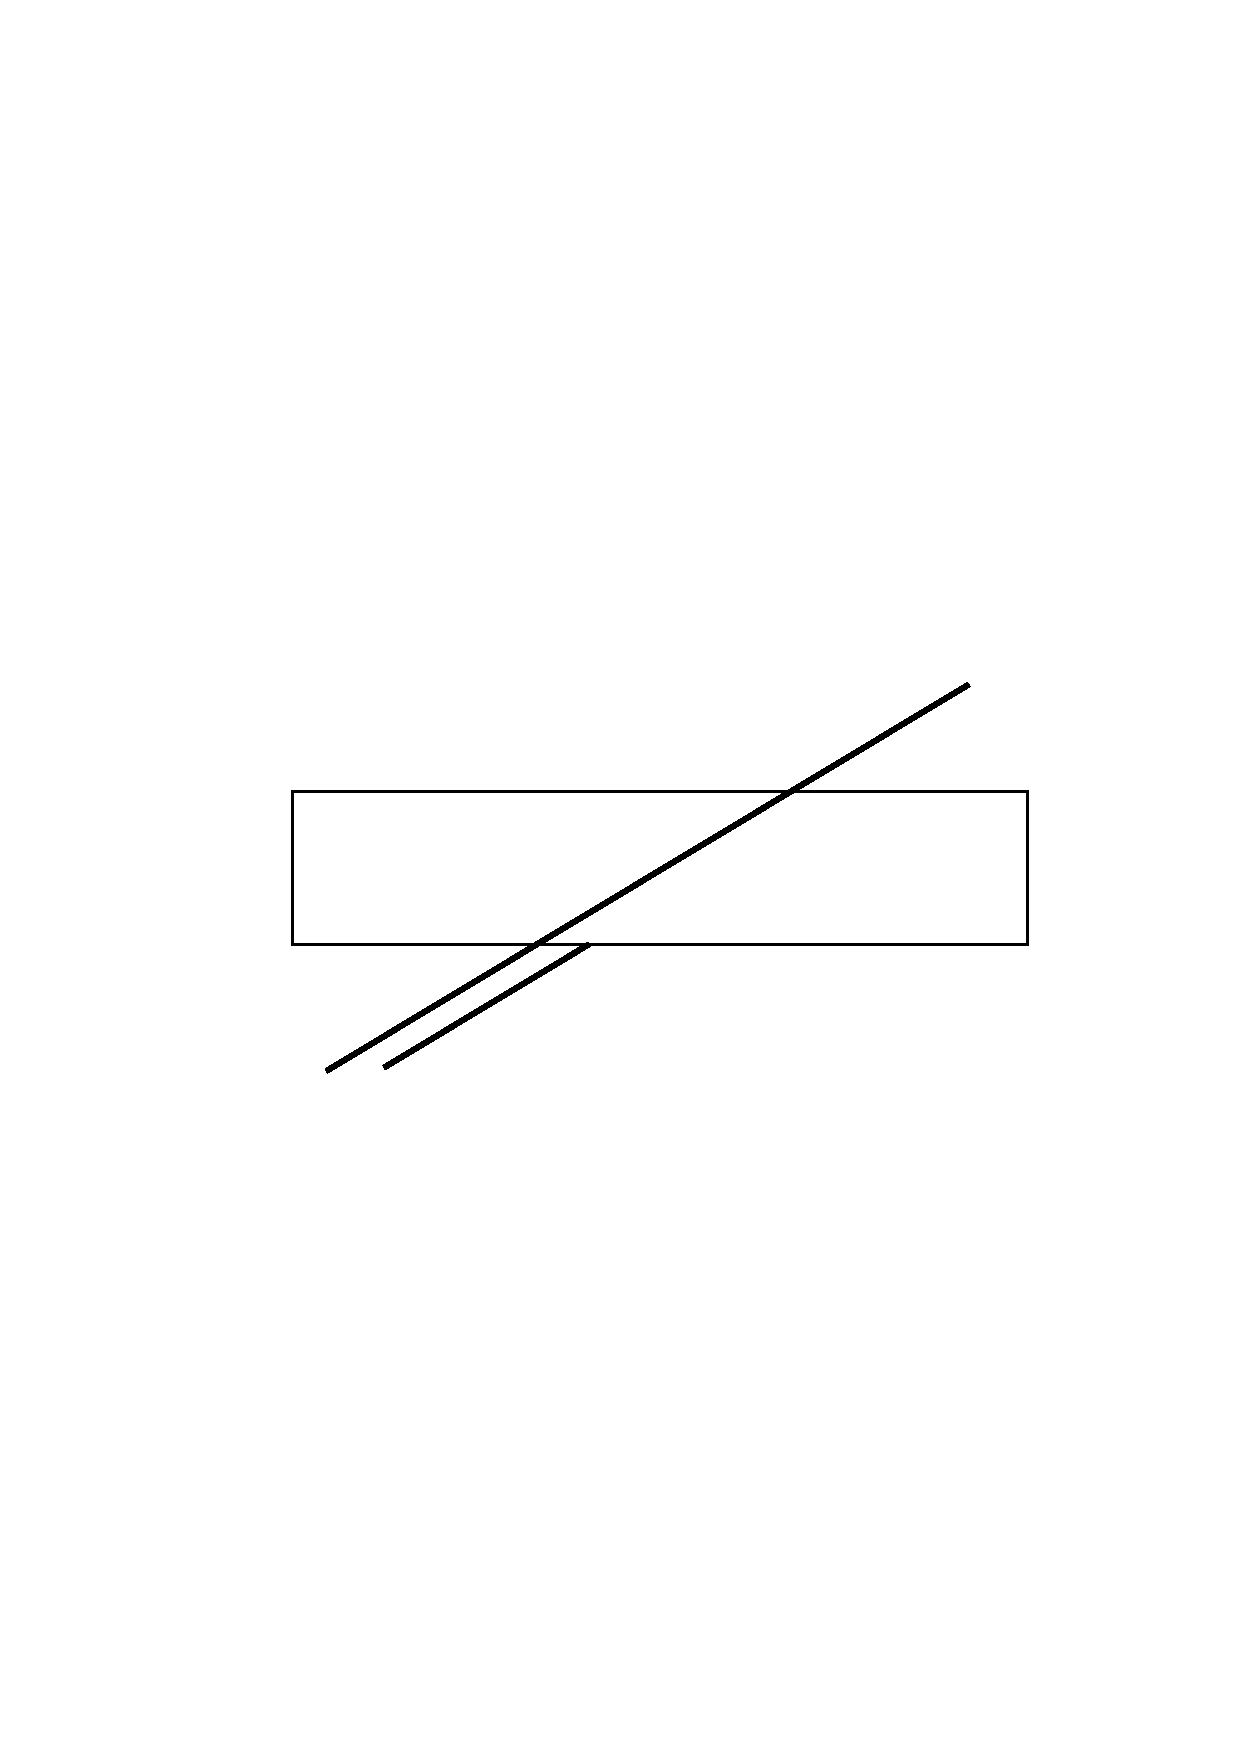
\includegraphics[width=9cm]{Images/optische_taeuscung_loesung2.pdf}
\end{figure}
     {\footnotesize  Poggendorff illusion}

}

%% --------
 \frame{
  \frametitle{}
 \url{http://www.youtube.com/watch?v=JhjUJTw2i1M}\\
 
     {\footnotesize  02:28 to 04:15}
}




%% --------
 \frame{
  \frametitle{Visual illusion}
	
	\begin{block}{}
	 \begin{itemize}
		\item Visual illusions give a wrong interpretation of data.
   		\item Do not create visual illusions, e.g. by making pie charts.
	 \end{itemize}

	\end{block}
}


%% --------Schlussfolgerung
 \frame{
  \frametitle{Tipps (if possible)}
\begin{itemize}
	\item Do not (accidentally) cause \textit{visual illusions} $\to$ leads to wrong conclusions.
	\item Do not use \textit{colors} or \textit{shades} if not necessary $\to$ difficult to decode (\url{colorbrewer2.org})
	\item Do not use \textit{areas} or volumes (e.g. 3D plots)  $\to$ difficult to estimate.
	\item When using areas, they should be \textit{proportional} to the actual values (e.g. circles).
	\item Do not only present graphs to the audience - also explain your data and your mapping technique.
	\item Do not use more \textit{dimensions} in a graph than you have data.
	\item Reduce the graph - every ink on a graph needs a \textit{reason} (data - ink - ratio)	
\end{itemize}
}

\section{Conclusion 1: Implementation in software}


%% --------
 \frame{
  \frametitle{R: software for statistics and computing}
\url{http://www.r-project.org/}
}

  %% --------
 \frame{
  \frametitle{2 purposes of visualizing data}
  	 \begin{block}{Purpose 1: analyse data}
       I only graph data for myself or some members of my research group.
	\end{block}
	
  	 \begin{block}{Purpose 2: graphs as communication}
	I produce graphs and show them to others (e.g. in an article).
	\end{block}
}

 \frame{
  \frametitle{}
  %% -------- 


 \begin{figure}[H] 
    \centering 
      \subfloat{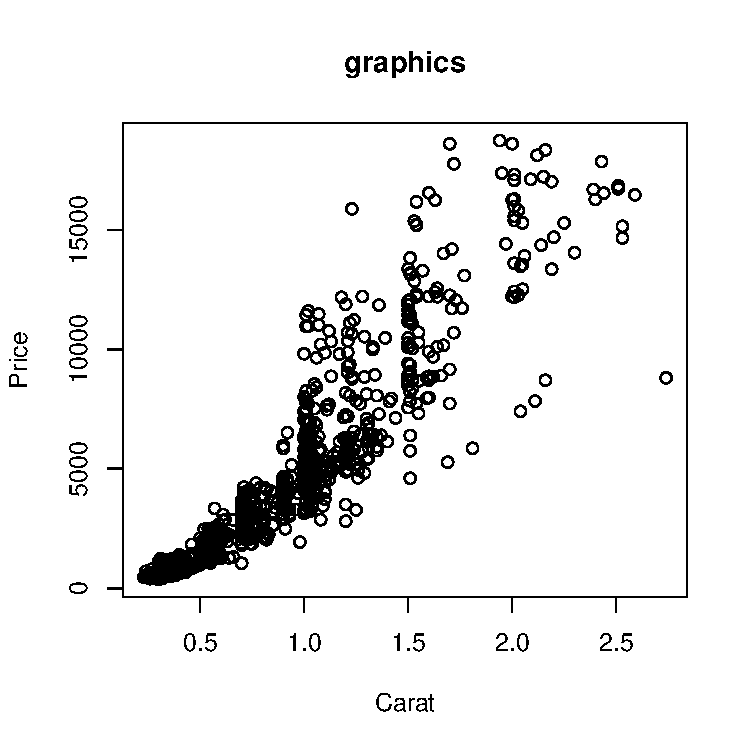
\includegraphics[width=4cm]{Images/xyplot_graphics_iris2.pdf}}
        \subfloat{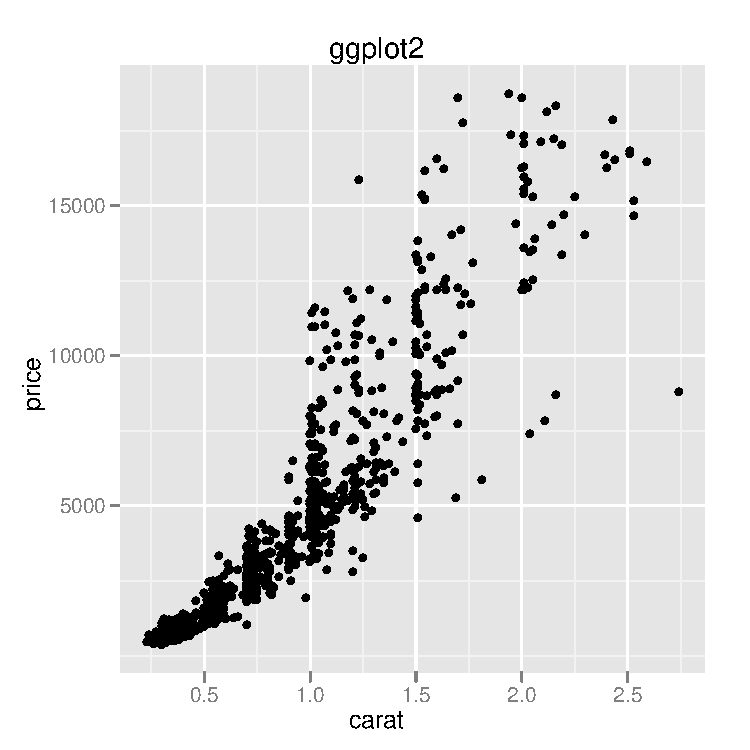
\includegraphics[width=4cm]{Images/xyplot_ggplot2_iris2.pdf}}
      \subfloat{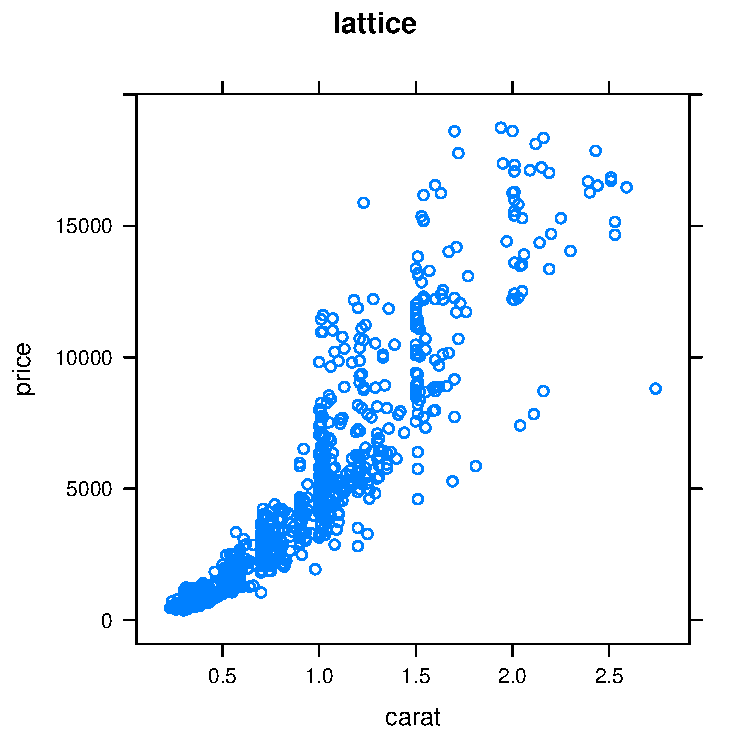
\includegraphics[width=4cm]{Images/xyplot_lattice_iris2.pdf}}
\end{figure}
	
}


%% --------
 \frame{
  \frametitle{}
 \begin{figure}[H] 
    \centering 
       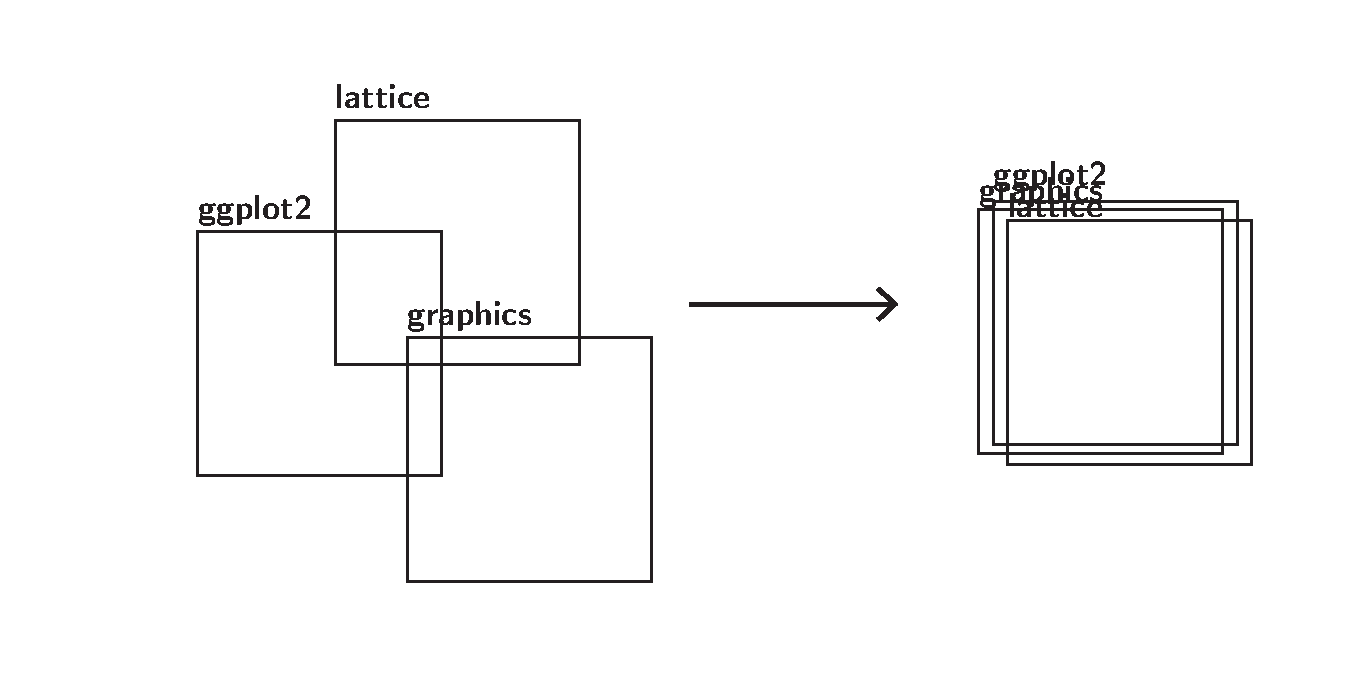
\includegraphics[width=12cm]{Images/package.pdf}
\end{figure}

}


\section{Conclusion 2: Recipes}


 \frame{
  \frametitle{}
 \begin{figure}[H] 
    \centering 
       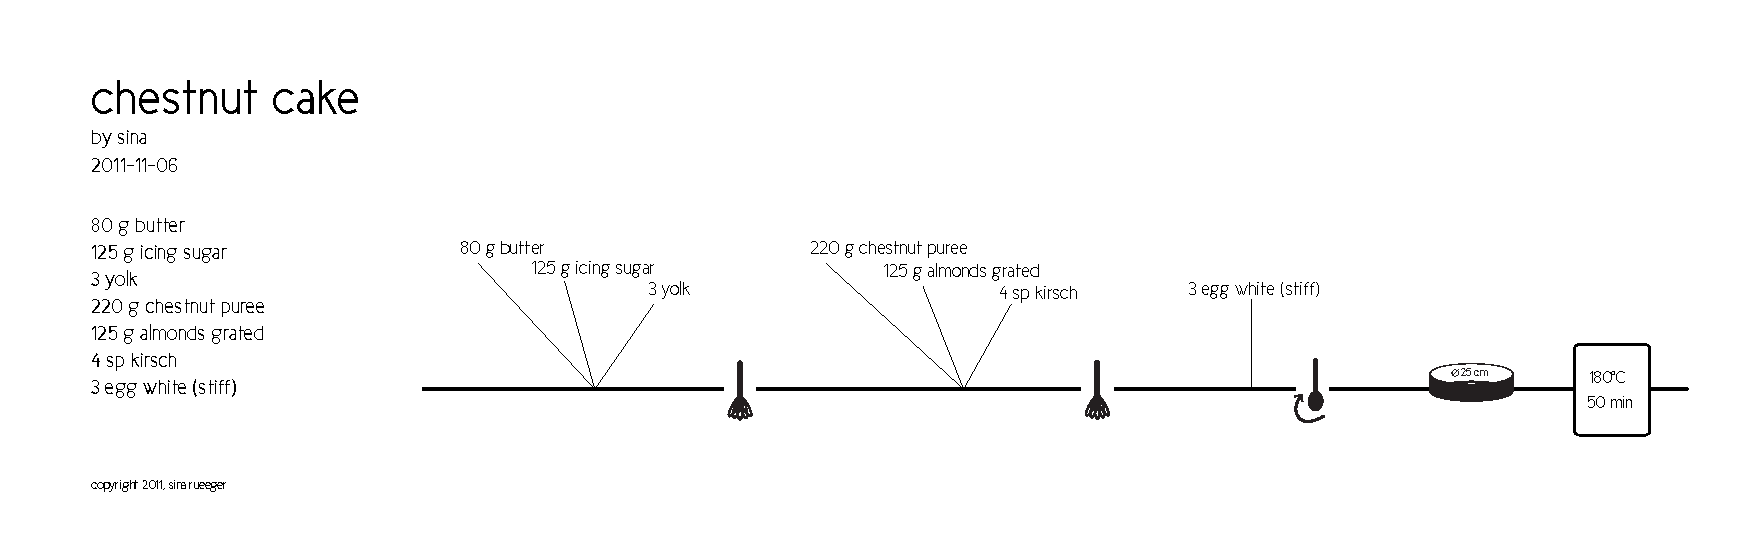
\includegraphics[width=12cm]{Images/chestnut_cake_ai.pdf}
\end{figure}
}

 \frame{
  \frametitle{}
 \begin{figure}[H] 
    \centering 
       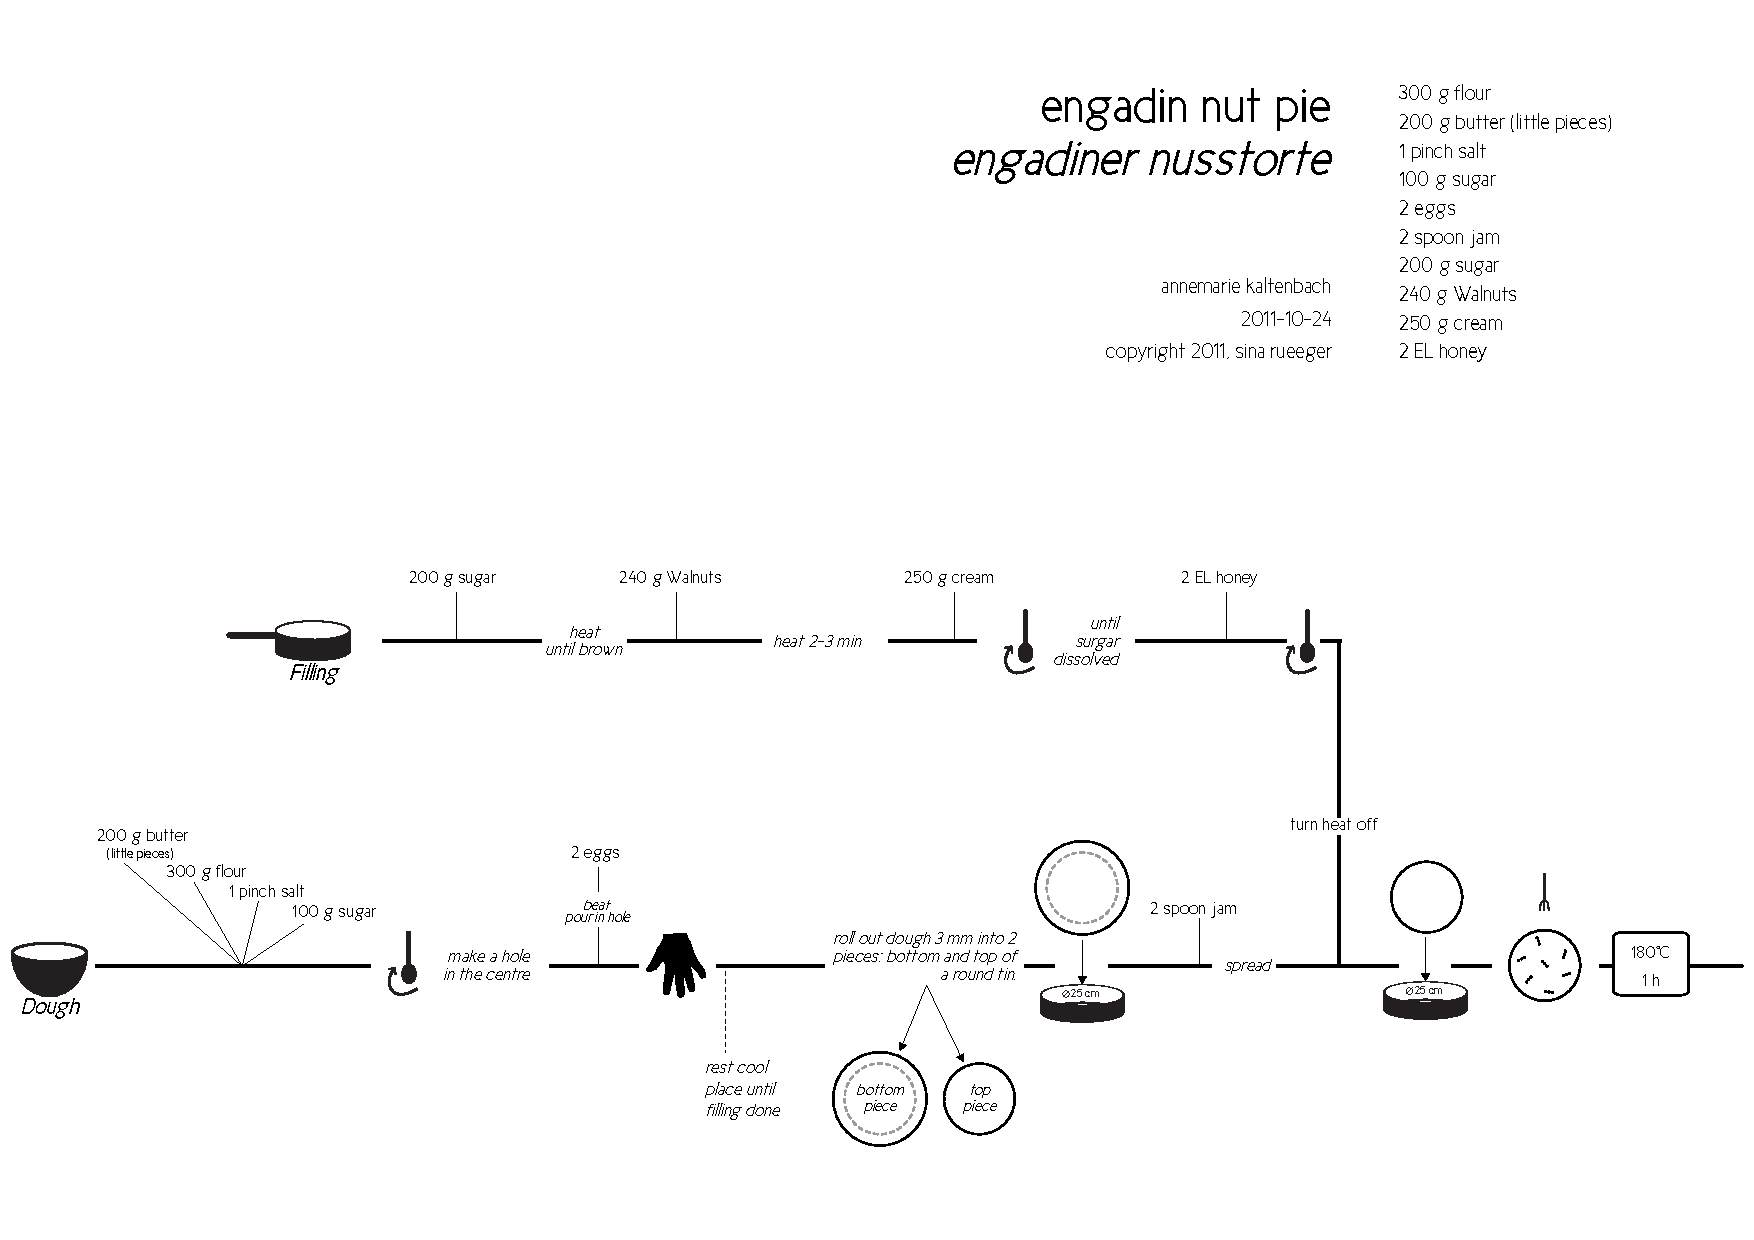
\includegraphics[width=10cm]{Images/nusstorte_ai_icons.pdf}
\end{figure}
}

%% ---
\frame{
  \frametitle{}
	\begin{block}{Edward Tufte in \emph{The Visual Display of Quantitative Information} (1995)}
	''Above all else show the data!''
     	
	''Data graphics should draw the viewers attention to the sense and substance of the data, not something else.''
      	
	\end{block}

  }
\end{document}
